\documentclass[tocnopagenum]{thesis-ekf}
%a4paper, 12pt, 1.5-es sortávolság, margók
\PassOptionsToPackage{defaults=hu-min}{magyar.ldf}
\usepackage[magyar]{babel}
\usepackage[T1]{fontenc}
\usepackage[utf8]{inputenc}
\usepackage{mathtools,amssymb,amsthm,pdfpages}
\footnotestyle{rule=fourth}
\usepackage{comment}
\usepackage{enumitem}
\usepackage{booktabs}
\usepackage{graphicx}
\graphicspath{ {./images/} }


\newtheorem{tetel}{Tétel}[chapter]
\theoremstyle{definition}
\newtheorem{definicio}[tetel]{Definíció}
\theoremstyle{remark}
\newtheorem{megjegyzes}[tetel]{Megjegyzés}

\begin{document}
	\institute{Matematikai és Informatikai Intézet}
	\title{Interfész megoldások imperatív és OOP nyelvek közötti kapcsolattartásra}
	\author{Nagy-Tóth Bence\\Szak: Programtervező informatikus BSc\\Specializáció: Szoftverfejlesztő informatikus}
	\supervisor{Dr. Király Roland\\beosztás}
	\city{Eger}
	\date{2022}
	\maketitle
	\tableofcontents
	
	\chapter*{Bevezetés}
	\addcontentsline{toc}{chapter}{Bevezetés}
	Az ember kognitív képességeinek fejlesztésére mindig is szükség volt, van és lesz is a jövőben. Ez a megállapításom különösen beigazolódni látszik egy COVID-világjárvány utáni időszakban, amikor is sorra jelennek meg olyan jelentések \emph{TODO referencia erre} \cite{brain1}, amelyek azt támasztják alá, hogy a lezárások ideje alatt nőtt a különböző mentális betegségek (többek között a demencia, \emph{TODO példák}) kialakulásának kockázata. Nem beszélve arról, hogy a digitális eszközök használata számtalan alkalommal hosszas órákon keresztül képes lekötni a figyelmünket, ezért bizonyos külső ingerekre egyre lassabban, kisebb amplitúdóval, azaz nagyobb közömbösséggel tudunk reagálni. A demencia, azaz a kognitív képességek leépülésének tünetei közé tartoznak a különböző beszédzavarok, az ítélőképesség és az elvonatkoztatás képességének romlása.
		\begin{figure}[h!]
		\centering
		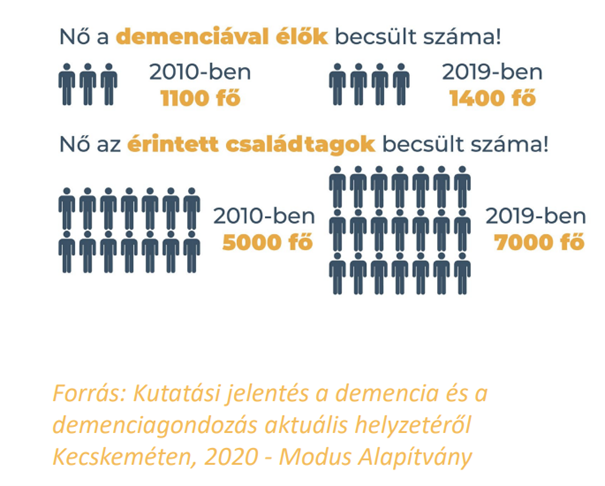
\includegraphics[scale=0.7]{images/demencia.png}
		\caption[caption]{\\\hspace{\textwidth}Forrás: saját szerkesztés}
		\label{fig:demencia}
	\end{figure}
	Az értelmi hanyatlást különféle egészségkárosító szokások -- például az alkoholfogyasztás -- szervi károsodás, akár ezek együttese is okozhatja, a legjelentősebb kockázati tényező ilyen téren azonban az ember életkora. 
	\begin{comment}
		TODO: FORRÁSOK!
	\end{comment}
	Szakdolgozatom ezen pontján azért érdemes erről a betegségről szót ejtenem, mivel alapvetően számomra már önmagában motivációul szolgál a tudat, hogy egy ilyen nagy volumenű elmélet megvalósításában vehetek részt, amely a demencia megelőzését, a mentális állapot folyamatos rongálódásának megfékezését célozza. 
	Az általunk készített szoftver támogatást nyújthat csoportfoglalkozásokon, tulajdonképpen egy tornaórát le tudunk vezényelni az eszközöknek köszönhetően. Természetesen az eszközök által kibocsájtott különböző fény- és hangjelzések önmagukban nem hordoznak semmiféle jelentést, a jelzések konkrét  a tornaórákat vezénylő szakemberek dolga közölni a csoport számára.
	\chapter{Programozási nyelvekről általában}
	\section{A programozási nyelvek formális nyelvek?}
	\begin{definicio}
		Legyen $\mathbb{A} = \{a_1, a_2, ... a_n\}$ véges, nemüres ($ \mathbb{A} \neq \emptyset$) halmaz, ezt a nyelv ábécéjének, elemeit betűknek vagy jeleknek nevezzük. $\mathbb{A}$ halmaz elemeiből képezzük annak hatványait, ekkor 
		\begin{enumerate}
			\item $\mathbb{A} ^ {0}$ az üres szó ($\epsilon$) egyelemű halmazát, 
			\item $\mathbb{A} ^ {1} $ az egybetűs szavak (\,$\mathbb{A}^{1}\subseteq\mathbb{A}\wedge\mathbb{A}\subseteq\mathbb{A}^{1} \iff \mathbb{A}^{1}=\mathbb{A}$\,), 
			\item $\mathbb{A}^{2}$ a kétbetűs szavak, 
			\item $\mathbb{A}^{n}$ az $n$ hosszú szavak halmazát jelenti és így tovább.
		\end{enumerate}
	Jelölje $A^{*}=A^{0}\ \cup\ A^{1}\ \cup\ A^{2}\ \cup\ \dots\ \cup\  A^{n}$ az ábécé elemeiből képzett véges szavak vagy más néven jelsorozatok halmazát (ezt az $\mathbb{A}$ ábécé feletti univerzumnak hívjuk). Ekkor  $\mathbb{A}$-ból kirakható szavak $\mathbb{A}^{*}$ halmazának egy részhalmazát \textbf{formális nyelvnek} nevezzük. Szokásos még az $\mathbb{A}$ ábécé feletti formális nyelv megnevezés is. A hatványok a halmaz önmagával vett \emph{Descartes-szorzatait} jelentik.
	\cite{formnyelvek}
	\end{definicio}
	
	Fő különbségek formális és természetes nyelvek között:
	\begin{itemize}
		\item A formális nyelveket egy dedikált célra hozzuk létre, ezeket általában nem használjuk interperszonális (emberek közötti) kommunikációra. Ezzel szemben egy természetes nyelv (például az angol) egy emberi közösség aktuális és a múltban használt jelkészletét rendszerezi.\\
		A C++ programozási nyelv például azért jöhetett létre Bjarne Stroustrup dán szoftverfejlesztő jóvoltából, mert a C - procedurális nyelv lévén - nem tette lehetővé többek között a tisztább objektum-orientált programozást, a memóriacímek helyett a biztonságosabb referenciák használatát. \cite{cpplang1}
		\item A formális nyelvek kulcsszavakból állnak. A természetes nyelvek több építőelemből tevődnek össze: fonémák (hangok, betűk), morfémák (szótövek, toldalékok), szavak, mondatok, bekezdések, szövegek.
		\item A természetes nyelvek fejlődhetnek spontán, emberi generációról generációra valamint tudatos módon (például nyelvújítás) egyaránt. A formális nyelvek alakulását egy tervezési fázis előzi meg, ekkor a nyelv szabályrendszerét lefektetik, tehát csak és kizárólag tudatos, mesterséges beavatkozással lehet megreformálni őket.
		\item Az ember által is beszélt természetes nyelvek esetén a használt szavak hangsúlyozásának, hanglejtésének, valamint a beszéd hangerejének is jelentésmódosító ereje lehet, a formális nyelvek esetében hangsúlyról egyáltalán nem beszélhetünk.
	\end{itemize} \cite{langvid1} \cite{langvid2}

	A fentiekből következően minden programozási nyelv formális nyelvnek számít. 
	\section{Jelenleg népszerű programozási nyelvek}
	2022-ben a legnépszerűbb programozási nyelveknek számítanak (a teljesség igénye nélkül):
	\begin{enumerate}
		\item JavaScript
		\begin{itemize}
			\item 1995, \textit{Brendan Eich} fejlesztette a webböngészési funkcionalitások kibővítése végett.
			\item web-, játék-, valamint mobilfejlesztésre egyaránt használják
			\item webszerverként is tud funkcionálni (Node.js)
		\end{itemize}
		\item Python
		\begin{itemize}
			\item 1991, \textit{Guido Van Rossum} tervezte annak érdekében, hogy olvashatóbb és nagyobb kifejezőerővel rendelkező kódok készülhessenek, a szintaktikai szabályok helyett a kód működésére tudjanak a programozók koncentrálni
			\item backend-fejlesztés
			\item automatizálás
			\item web scraping\footnote{Információgyűjtés eszköze, amely lehetővé teszi, hogy automatizált módon (kód segítségével) bizonyos weboldalakról tetszőleges adatokat (például posztokat, közelgő eseményeket) letölteni.}
			\item Data Science\footnote{Az informatika, a matematikai statisztika és az üzleti elemzés metszetében álló tudományág, amely adatok összegyűjtésével, ezek elemzésével foglalkozik annak érdekében, hogy a vállalatok jobb üzleti döntéseket tudjanak meghozni ezek segítségével. \hyperref{https://qr.ae/pvlYmQ}{}{}{Forrás}}
		\end{itemize}
		\item HTML
		\begin{itemize}
			\item webdokumentumok kezelése: JSON, XML, SVG
			\item weboldalak statikus (állandó) részeinek fejlesztése
		\end{itemize}
		\item CSS 
		\begin{itemize}
			\item weboldalak formatervét, kinézetét, stílusát alakítja ki
			\item HTML mellett hívják segítségül
		\end{itemize}
		\item Java
		\begin{itemize}
			\item 1995, Sun Microsystems fejlesztése, alapötlet: olyan eszközök vezérlése, amelyek elférnek egy kézben
			\item E-kereskedelem
			\item Financial Technology: pénzintézetekkel, tőzsdékkel, számlázással kapcsolatos szoftvereket jellemzően ezen a nyelven fejlesztik
			\item a megírt kódok futtathatóak különösebb átalakítás nélkül az elterjedtebb operációs rendszereken (a kód hordozható, platformfüggetlen)\footnote{Ez azért lehetséges, mivel .exe fájl helyett egy átmeneti .class állomány (bytecode) készül, amit egy virtuális gép (Java Virtual Machine) tolmácsolja (interpretálja) gépi kódként a számítógépünknek \hyperref{https://www.upgrad.com/blog/why-is-java-platform-independent-language/}{}{}{Forrás}}
		\end{itemize}
		\item SQL
		\begin{itemize}
			\item 1972, \textit{Donald D. Chamberlin} és \textit{Raymond F. Boyce} az IBM alkalmazásában, adattáblák egyszerűbb kezelésének érdekében hozták létre
			\item adatbázisok kezelése, karbantartása
			\item Data Science
		\end{itemize}
		\item Go
		\begin{itemize}
			\item 2009, a Google fejlesztői alakították ki, hogy megoldják a hatalmas szoftverrendszerekkel kapcsolatos problémákat
			\item rendszerek, hálózatok programozása
			\item hang- és videószerkesztés
			\item Big Data\footnote{Az informatika egyik tudományága, amely tömérdek mennyiségű, hagyományos számítógéppel nehezen kezelhető adatok tárolásával és feldolgozásával, ezek elemzésével foglalkozik.\hyperref{{https://www.youtube.com/watch?v=bAyrObl7TYE}}{}{}{Forrás}}
		\end{itemize}
		\item C
		\begin{itemize}
			\item 1970-es években Ken Thompson és Dennis Ritchie jóvoltából, Assembly-nél magasabb szintű (természetes nyelvezethez közelebb álló) nyelv kialakítása volt a célja
			\item hardverelemek illesztőprogramjai, vezérlőkódjai
			\item operációs rendszerek fejlesztése
			\item 3D videók szerkesztése
			\item alacsonyabb szintű a fentebb felsoroltaknál, ezért könnyebb optimalizálni memória és futásidő szempontjából
			\cite{clang1}
		\end{itemize}
	\end{enumerate}\cite{proglanguages1}\cite{proglanguages2}
	
	\chapter{Marshalling}
	\section{Milyen adatszerkezeteink vannak?}
	A programozási nyelvek szintaktikában ugyan eltérnek egymástól, amikor viszont adatok tárolásáról van szó, egy dologban egyetértenek: típusokra szükség van. Mit jelent az, hogy egy változót például \verb*|bool| típusúként definiálunk? Az adat típusa meghatározza, hogy
	\begin{itemize}
		\item mekkora memóriaterületet\footnote{mivel a byte számít a legkisebb megcímezhető memóriaegységnek, ezért ennek mértékegysége alapértelmezetten bájtban értendő} kell számára lefoglalni
		\item a számítások folyamán hogyan kell őt értelmezni\\(például ha másik változónak értékül adjuk, hány bitet kell másolni)
		\item továbbá milyen műveletek végezhetőek vele\\(például egész típusú változókon értelmezhetjük a szorzás műveletét, szövegeknél ezt már nem tehetjük meg).
	\end{itemize} \cite{adatszerkezetek_88}
	\section{Használt adatszerkezetek}
	Ahogy említettem, a programozási nyelvek döntő része típusos, ezenfelül kisebb-nagyobb különbséggel hasonló adatszerkezeteket értelmez.
	\begin{enumerate}[label=\alph*)]
		\item \emph{elemi adattípusok}: Olyan típusok, amiket nem tudunk további részekre bontani, csak egyben értelmezhetjük őket. Ilyen például a \verb*|double| lebegőpontos típus, amely 8 bájton képes lebegőpontos számot ábrázolni. Igaz, hogy csak az első bájtra van mutatónk, de nincs értelme további bájtokra darabolni, és megnézni az értékeket, mivel egyben értelmezendő, a műveleteket 4 byte-on fogjuk tudni vele végezni. Primitív adattípusoknak is nevezzük őket.\\
		Vegyük például a C\# programozási nyelvet, milyen elemi típusai vannak?
			\begin{enumerate}
				\item egész:
				\begin{tabular}{ccc}
					Előjeles típus & Előjel nélküli típus & Méret (bájt) \\
					sbyte & byte & 1 \\
					short & ushort & 2 \\
					int & uint & 4 \\
					long & ulong & 8 \\
				\end{tabular}
				\item lebegőpontos:
				\begin{tabular}{cc}
					Típus neve & Típus mérete (Bájt) \\
					float & 4 \\
					double & 8
				\end{tabular}
				\item logikai: 
				\begin{tabular}{cc}
					bool & 1 Bájt
				\end{tabular}
				\item karakteres: 
				\begin{tabular}{cc}
					char & karakterkódolástól függ\footnote{ASCII kódolás esetén egyetlen karakter 7, míg UTF-8 kódolás esetében 8 biten tárolódik. Mivel a legkisebb megcímezhető egység az 1 bájt, ezért ezek 1 bájt területet foglalnak karakterenként, ASCII-kód esetében a 8. bit értékét nem veszik figyelembe. 
					Ezzel szemben az újabb UTF-16- és UTF-32-szabványok esetében az előbbiben 2 bájt, utóbbiban 4 bájt memóriaterület szimbolizál egyetlen karaktert.}
				\end{tabular}
			\end{enumerate}
	\item \emph{összetett adattípusok}: Az összetett adattípusok elemi típusokra szedhetők szét, vagyis primitív és/vagy további összetett típusú változókból épülnek fel. Ami a adattagok vagy mezőnek nevezzük. Az összetett adattípusú változók tárolásához szükséges memóriaterület kiszámítható az adattagjainak összegével.\\
	C\#-ban a \verb*|struct| és a \verb*|class| kulcsszavakkal tudunk összetett típusokat definiálni.
	\end{enumerate}
	\section{Mi a helyzet az algoritmusokkal?}
	Adatokat tudunk tárolni, és ezt tesszük azért, mert tervünk van velük, azaz valamit szeretnénk velük kezdeni. Az adatszerkezeteken végzett véges számú elemi lépéssorozatot algoritmusnak nevezzük. Az adatszerkezetek algoritmusok nélkül lényegében olyanok, mint a matematikai műveletek operátorok (összeadás, kivonás, stb.) nélkül, végül -- ha már említettem a természetes nyelveket-- mint a főnevek igék nélkül.
	\section{Kommunikáció adatszerkezeteken keresztül}
	A \emph{Marshalling} egy olyan folyamat, amely összetett típusok átalakítására szolgál, hogy egy nyelv adatszerkezetét a másikkal megértessük. Magyar fordításával nem találkoztam ennek a kifejezésnek, de leginkább talán az 'átalakítás' szóval tudjuk leírni, ami adatszerkezetek esetében annyit tesz, hogy más nyelv által is értelmezhetővé tesszük, kevésbé hagyatkozunk az adott nyelv különlegességeire.
	\par
	A Marshalling sajnos nem minden esetben szolgáltat tökéletes megoldást, szakdolgozati projektünkön keresztül például látni fogjuk, hogy a kód további portolhatósága, újrahasznosíthatósága végett megéri szabványos formátumokon keresztül kommunikálni, mint azt tesszük API-k\footnote{TODO: API leírása...} vagy konfigurációs fájlok esetében \footnote{Például az \textit{app.config} fájl a C\#-ban XML-formátumban látható.}, ilyenek például az általam használt JSON- vagy XML-formátumok,  hogy más felületekre való költöztetés esetén kompatibilitási probléma többé már ne merülhessen fel.
	A Marshalling primitív típusok esetén abszolút működőképes, összetett adatszerkezetekre viszont inkább a szabványos szöveges formátumokat érdemes alkalmazni tapasztalatom szerint. Ha ezt elfogadjuk, akkor érdemes megismerkedni a szerializáció és deszerializáció 
	\section{Mik a stubok?}
	A stubok hívó (aki csak az implementált metódus fejlécét\footnote{A fejlécet szignatúrának is nevezzük: ez a metódus visszatérési típusát (a \emph{void} is visszatérési típusnak számít), nevét és paraméterlistáját együttesen teszi ki}) és a hívott (ahol a két kód szerződésében lévő publikus/,,meghirdetett''/exportált metódusok -- és még akár továbbiak is -- implementálva vannak) fél között elhelyezkedő mini egységek.
	
	\chapter{Szakdolgozati projektünkről}
	A szakdolgozat mellé készített projektemet Sipos Levente hallgatótársammal fejlesztjük. Munkánk arról szól, hogy Keresztes Péter tanár úr által Delphiben implementált metódusokat hívunk meg C\#-os környezetben. A C\# és Delphi nyelvek összehangolása az én feladatom, az elkészült termék terveim szerint úgynevezett Helper-metódusok implementációit tartalmazó, lefordított\footnote{Lévén a C\# fordított nyelvnek számít, ezért az alkalmazások futtatásához/használatához az elkészült forráskódokat első lépésben futtatható állományra (gépi kódra) kell fordítani egy fordítóprogram segítségével. Ezt a folyamatot szakszóval \textit{compilingnak} vagy \textit{buildelésnek} is nevezzük.} DLL projekt lesz C\# nyelven, amelyeket Levente az ő grafikus alkalmazásában tud meghívni. A projekt jelen állása szerint szükség volt továbbá egy úgynevezett relayDLL-re, amelyet én állítottam össze.
	\section{Miről is szól a projektünk?}
	
	Egy mentális egészségfejlesztésre használatos alkalmazást fejlesztésére vállalkoztunk 2022 szeptemberében, amely elméleti alapjait Somodi László futballedző munkásságának köszönhetjük, ezek technikai részleteiről titoktartási szerződésünk
	\begin{comment}
	TODO: Ezt akár betehetnénk ide vagy hivatkozhatnánk rá
	\end{comment}
	lévén csak nagyon érintőlegesen fogok beszámolni a későbbiekben. 
	
	A készített alkalmazásunk gyakorlatilag különböző fény- és hangjelzések kibocsátására alkalmas eszközök (több LED-ből felépülő lámpák, nyilak és hangszórók) vezérléséből áll, egy ún. \emph{intelligens szobában} az eredeti tervek szerint 8 eszköz (a készített program azonban tetszőleges, $n$ darabszámú eszköz vezérlésére lett felkészítve) együttes vezérlését kell kezelnünk megadott időközönként (ezeket ütemnek fogjuk nevezni). A program azzal indít, hogy felméri az USB-porton csatlakoztatott, egymással RJ11-csatlakozókkal sorba kötött eszközöket, őket a típusának megfelelő azonosítóval látja el. Az azonosító meghatározza, hogy egy eszköz milyen típusú. 
	
	Egy feladatsor több egymást követő ütemből áll, mely a programban azt fogja jelenti, hogy x másodperc késleltetéssel a felmért eszköz tömb elemeinek tulajdonságait (mezőit) a feladatsor aktuális ütemének megfelelően módosítjuk. Mivel minden eszközt együttesen vezérlünk, a program ütemenként az összes eszköz állapotát felül fogja írni, ezért szükségünk van egy olyan állapotra is, ami azt közli az adott eszközzel, hogy éppen semmit ne csináljon (azaz várakozzon). Ez a fényeszközök esetében egyszerűen (0,0,0) RGB-színkód\footnote{Az RGB-színkódolás egy szín leírását három komponens, vörös (\textbf{R}ed), zöld (\textbf{G}reen) és kék (\textbf{B}lue) alapszínek arányától teszi függővé.} közlését, míg hangeszköz esetén egy 0 dB hangerősségű tetszőleges frekvenciájú hangjelzés kiküldését fogja jelenteni.
	Somodi László edzővel való együttműködésünk Dr. Király Roland tanár úr jóvoltából jöhetett létre, akinek az alkalmazással kapcsolatos múltbéli tapasztalatait és  ötleteit folyamatos egyeztetések, konzultációk útján tudtuk segítségül hívni.
	\section{Delphi és C\# programozási nyelvek összehasonlítása}
	Először is érdemes leszögeznünk, hogy a továbbiakban Delphi alatt nem a fejlesztői környezetet, amely az Object Pascal nyelvvel dolgozott együtt, hanem inkább a programozási nyelvet értjük, jelenleg az Object Pascal megnevezés úgynevezett ,,umbrella term'' formájában él tovább.\footnote{Az umbrella term (magyarul gyűjtőfogalom) olyan kifejezés, amely több fogalmat rendel önmaga alá, így már fogalmak egy csoportját, kategóriáját jelenti összefoglalóan.} \cite{sof_delphi}
	
	A Delphi nyelv (megjelenési éve: 1986, a Borland nevű cég jóvoltából) idősebb nyelvnek számít a C\#-hoz (megjelenési éve: 2001, a Microsoft 
	jóvoltából) viszonyítva, ebből fakadóan egy stabilabb, kiforrottabb, időtállóbb eszköznek számít a programozók kezében. 
	
	Mindkét nyelv \textbf{objektumorientált}, ami azt jelenti, hogy bizonyos, logikailag összetartozó adatokat (mezőket), valamint a rajtuk végezhető műveleteket (metódusokat) egy egységbe zárunk, ezt az egységet a továbbiakban osztálynak nevezzük. Az osztály mezőit és metódusait különböző láthatósági szintekkel vértezhetjük fel, ezzel tudjuk védeni az osztályunk kritikus részeit más osztályokkal szemben. Az osztályok között akár öröklődéssel akár objektum-összetétellel viszonyokat alakíthatunk ki.
	
	A két nyelv \textbf{erősen típusosnak} számít, mivel egy változó definiálásakor meg kell mondanunk azt is, hogy milyen típusú értékeket szeretnénk abban tárolni, a típusok már a forráskódban explicit módon megjelennek, így az adott nyelv fordítóprogramja fel van készítve a változó típusaira, amely változó hatókörén\footnote{Hatókör, illetve \textit{scope} alatt a program azon részét, kontextusát értjük, amely magába foglalja az adott változót. Ezen kontextusban vizsgálva a változó "életben van", tehát a memóriában hely van lefoglalva számára, nevére vagy memóriacímére hivatkozva értékét felülírhatjuk, kiolvashatjuk.} belül nem is változhat meg. Ahogy azt már korábban is említettem, a változó típusa meghatározza, hogy az értéket hogyan kell értelmezni a memóriában, a megadott típusnak mely műveletei vannak értelmezve, így például \verb|string| típuson nem értelmezhetünk logikai ÉS (konjunkció)-műveletet.
	
	Az elkészült kódok teljesítménye alapján is érdemes összehasonlítani a két nyelvet. Ehhez először is külön kell választanunk a fordításhoz és a futtatáshoz szükséges időt, lévén ezek fordított (nem interpretált) nyelvek, ezért ezek nem szimultán módon\footnote{nem egyidőben, nem egyszerre} történnek. A Delphi fordítóprogramja azonnal gépi kódot\footnote{A gépi kódban már az utasításokat is számok jelzik, ezen nyelv utasításkészlete már a számítógépben működő processzor típusától is erősen függ. Gépi kód az esetek nagy részében fordítóprogram eredménye, a hardverközeli vezérlőprogramok elkészítéséhez is inkább a magasabb szinten álló Assembly nyelvet használják.} készít, míg a C\# esetében első lépésben egy köztes nyelvű\footnote{A(z) (Common) Intermediate Language a .NET-keretrendszerben a magasabb absztrakciós szintű C\# és a legalacsonyabb szintű gépi kód között helyezkedik el, ami még processzortól és operációs rendszertől független. A .NET Runtime futtatókörnyezete képes futtatni.} kód készül, amelyet a .NET virtuális gép képes futtatni. Fordítási időben a Delphi-kód nyertesnek számít, futásidőben azonban közel ekvivalens a két nyelv révén gyártott kód.
	
	Ha ennél is tovább megyünk, akkor a C\#-nak nagy előnye származik abból a Delphivel való összevetésben, hogy aszinkron\footnote{ Az aszinkron programozás lehetővé teszi, hogy az alkalmazás egy időigényes folyamat futtatását háttérbe helyezze, így a programot futtató szál, lévén nem várakozik a válaszra, addig ugyanúgy képes a felhasználói interakciókat kiszolgálni. \cite{async}} kódolási lehetőséget is biztosít, amely felgyorsítja a végrehajtást, jobban ki tudja használni a rendelkezésre álló CPU teljesítményét. A LINQ\footnote{A \textbf{Language Integrated Query} (magyarul: nyelvbe ágyazott lekérdezés) egy gyűjtőfogalom a C\# nyelvbe épített szintaktikai elemekre, amely elemek lehetővé teszik, hogy akár lambda kifejezésként, akár SQL-szintaxishoz hasonló módon meg tudjunk fogalmazni lekérdezéseket bizonyos - iterálható, vagyis bejárható, az IEnumerable-interfészt megvalósító - szerkezetekre. Ilyen szerkezetnek minősül például a \textit{List} is.} használata \verb|yield| kulcsszóval az iterációkban biztosítja, hogy csak akkor van végrehajtva a kód, amikor ténylegesen szükség van rá (lusta kiértékelés). A delegate-ek használata szintén növelheti a C\#-kódok teljesítményét, bár a Delphi is rendelkezik ehhez hasonló funkciókkal.
	\begin{comment}
	TODO: esetleg ide jöhetne egy C\# és Delphi futásidő-összehasonlítási ábra (benchmark)
	\end{comment}
	\cite{perf_comp}
	
	A fejlesztés folyamán elkészített \textbf{modulokat} a különböző programozási nyelvek eltérő megnevezéseket használnak.\footnote{Az említett példákon kívül a Java-nyelvben \textit{package}-ként, míg a Pythonban \textit{module}-ként hivatkoznak az osztályokat összegyűjtő egységre.} A vizsgált két nyelv tekintetében is ez áll fenn: a C\# \verb|namespace|, míg a Delphi \verb|unit| kifejezéssel illeti, a lényegük ugyanaz lesz: 
	\begin{enumerate}
		\item Mivel nagy projekteknél előfordulhat, hogy két, funkciójában eltérő osztálynak ugyanazt a nevet kellene adnunk, nem tehetnénk meg, mivel a fordítóprogram, így a futó program sem tudná eldönteni, hogy a két változat közül éppen melyiket kívánjuk használni. Ezt a problémát orvosolják például, hogy külön modulokban tudjunk azonos elnevezésű osztályokat kezelni.
		\item Fontos továbbá, hogy mivel nem az nagyobb átláthatóság végett nem egy fájlban dolgozunk, és esetleg több kollégával fejlesztünk 
		\item Egy lefejlesztett DLL tekintetében is szükség van egyetlen összefoglaló névre, amit a futtatható állomány
	\end{enumerate}
	
	Ami közös még a két nyelvben, hogy a fejlesztés moduljaiból Win32 szabványnak megfelelő DLL-ek készülhetnek a segítségükkel, ezek szintén lefordított, gépi kódú állományok, amelyek más szoftver forráskódjában felhasználhatóak, lényegében így válnak futtatható állománnyá.
	\section{Alaphelyzet}
	Amikor a munkát megkezdtem, rendelkezésemre állt Dr. Király Roland tanár úr által fejlesztett Delphis asztali alkalmazás, amely -- mint kiderült -- a mai napig teljesen használható. Ezen alkalmazás forráskódjában követtem végig az hardvereket működtető függvények hívási sorrendjét (szekvenciáját), ezek mikéntjét és eredményeit. Ezen alkalmazás C\#-nyelvű megfelelőjének elkészítését és továbbgondolását kaptuk feladatként.
	\section{DLL-függvények bemutatása}
	A következőkben a Keresztes Péter tanár úr által Delphiben implementált metódusokat, ezek kezelésének lehetőségeit fogom részletezni.
	Általánosságban elmondható, hogy minden függvény egész típusú értékkel tér vissza, amely érték tájékoztat a lefutás eredményességéről: amennyiben a hívott metódus sikeresen (hiba, kivétel nélkül) lefutott, 0-val tér vissza, ahogy ezt egyébként az operációs rendszerek processzeinél is megszokhattuk. Ettől eltérő értékek az egyes hibatípusokat hivatottak meghatározni a Win32-szabvány\footnote{A Win32-es hibakódok szabványa szerint minden hibakódnak a $0x0000$ (decimálisan: 0) és $0xFFFFFF$ (decimálisan: $16\,777\,215$) közötti tartományban kell lennie.} keretein belül. Ezen hibakódok projektünkre vonatkozó részét az alábbi táblázatban \ref{fig:errcodes} összegyűjtöttem.
	\subsection{DLL megnyitása}
	A program indulásakor elsőként lefutó \verb*|SLDLL_Open| függvényt hívva elkezdhetjük az SLDLL további metódusainak használatát.
	\subsection{Eszközök felmérése}
	\verb*|SLDLL_Felmeres|
	\subsection{Hibakódok}
	\begin{figure}[h!]
		\hspace*{-1in}
		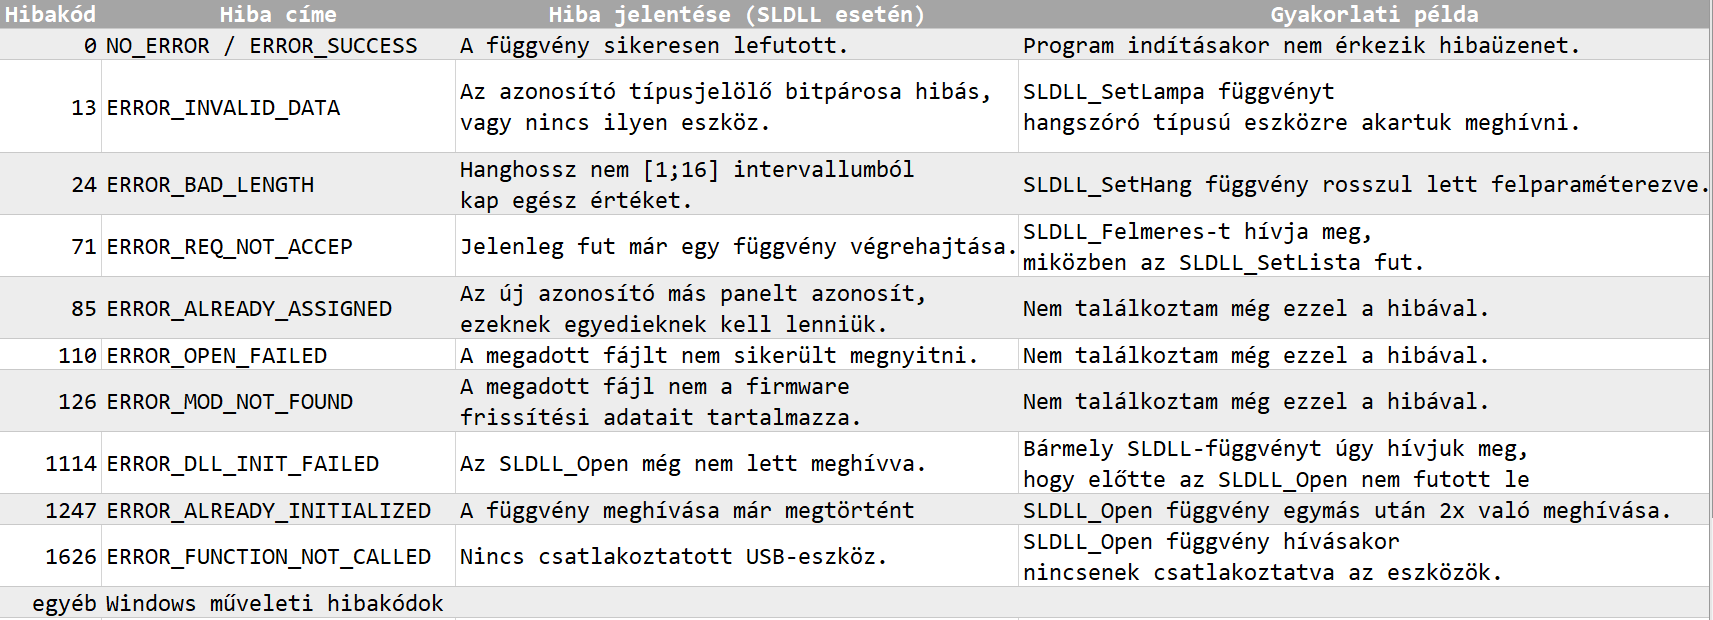
\includegraphics[scale=0.7]{images/errcodes.png}
		\caption[caption]{Win32-hibakódok magyarázata\\\hspace{\textwidth}Forrás: saját szerkesztés}
		\label{fig:errcodes}
	\end{figure}
	\cite{errcodes}
	Ezen hibakódokat C\#-ban megfelelő, egyénileg definiált kivételekkel, és sokkal kifejezőbb üzenetekkel váltom fel. 
	\subsection{A WinForm bemutatása}
	A \textit{WinForm}, teljes nevén a \textit{Windows Forms} a .NET GUI-fejlesztést\footnote{A GUI a Graphical User Interface (grafikus felhasználói interfész) kifejezés rövidítése, asztali alkalmazásokat értünk alatta, amely átlagfelhasználók számára kényelmesebb megközelítés a konzolos alkalmazásokkal szemben} támogató keretrendszere, amelynek segítségével egy asztali alkalmazást egyszerűbb módon el tudunk készíteni. 
	
	Előkészített, a HTML-nyelvből már jól ismert, valamint ezek tárházát bővítő vezérlőelemekkel (gombok, legördülő listák, adattáblázatok, és így tovább) gondoskodik azok újrahasznosíthatóságáról. A Visual Studio fejlesztői környezet egy Designer-felülettel is rendelkezik, amellyel gyorsan és különösebb képzelőerő nélkül elkészíthetjük grafikus alkalmazásaink vázát.
	
	Egy Windows Forms alkalmazásban a \textit{Form} (továbbiakban űrlapnak is fogom nevezni) egy vizuális felület,amely információkat jelenít meg a felhasználó számára.Egy Windows Forms alkalmazás általában úgy készíthető el, hogy egy Formhoz vezérlőelemeket (Control) adunk,a felhasználó által végrehajtott műveletekre, például egérkattintásokra és billentyűleütésekre adott válaszokat implementálunk. A \textit{vezérlőelem} különálló GUI-elemek gyűjtőfogalma, amely adatokat jelenít meg vagy adatokat fogad bevitelre.
	
	Amikor a felhasználó műveletet hajt végre egy űrlapon vagy annak vezérlőelemein, ez a művelet eseményeket generál. Az alkalmazás kódban reagálhat ezekre az eseményekre, amennyiben azok bekövetkeznek, de figyelmen kívül is hagyhatja azokat.\cite{winform}
	\subsection{DLL-ek üzenetküldése Win32-ben}
	Van egy üzenetlista\footnote{A Message Queue (üzenetsor) egy sor (queue) adatszerkezetben, érkezési sorrendben tárolja az üzeneteket, majd ezek ugyanezt a sorrendet megtartva kerülnek le róla.}, amin keresztül kommunikál az operációs rendszer a futó programmal, ezt projektünk szempontjából Levente ablakos alkalmazása fogja jelenteni. Az operációs rendszer ráteszi a lenyomott gomb által kiváltott üzenetet erre a listára, tehát például amikor az egér bal gombjával kattintunk,	akkor azt ténylegesen nem a futó program fogja észlelni, mivel az operációs rendszer a központ, ahova az I/O-kérések befutnak. \footnote{Az operációs rendszer eleve azért felelős, hogy elossza az erőforrásokat és kezelje a kimeneti-bemeneti perifériákat, így az egerünk által kiadott jel is az operációs rendszerhez érkezik be.}
	Az alábbi lépéssorozat fog lejátszódni:
	\begin{enumerate}
		\item Az operációs rendszer ráteszi a \verb*|WM_LBUTTONDOWN|-üzenetet az üzenetsorra.
		\item A programunk meghívja a \verb*|GetMessage|-függvényt.
		\item A \verb*|GetMessage| leveszi a \verb*|WM_LBUTTONDOWN|-üzenetet az üzenetsorról, és az érkező információkból feltölti a Message-adatszerkezetet.
		\item A programunk meghívja a \verb*|TranslateMessage|- és \verb*|DispatchMessage|-függvényeket, utóbbiban az operációs rendszer meghívja az asztali alkalmazás WndProc-függvényét Ez minden esetben lezajlik, attól függetlenül, hogy az ki van-e fejtve vagy sem.
		\item Az ablakos alkalmazásban válaszolunk az I/O-kérésre (például egy gombra kattintva újabb ablakot nyitunk meg) vagy éppen figyelmen kívül is hagyhatjuk, ekkor a felhasználó belátja, hogy lényegében nem is történt semmi.
	\end{enumerate}
	Már az is Win32-üzenetet vált ki, ha szimplán mozgatjuk az egerünket, ekkor az egér új pozíciója is az üzenetben tárolásra kerül, innen és a Form előre meghatározott tulajdonságaiból (pozíció, ablak szélessége és magassága) tudjuk detektálni például, hogy az egér az ablak területére érkezett\footnote{Erre vonatkozó esemény a MouseEnter-event Windows Form esetében.}.
	Ha erre a felhasználói bemenetre fel van készítve a programunk által üzenetküldésre használt metódus\footnote{Egy-egy Win32-üzenet feldolgozását Windows Form asztali alkalmazás esetében a WndProc-metódus szolgálja.}, akkor az érzékeli, hogy erre az eseményre reagálnia kell, így egy másik állapotba lép. Természetesen a készített programban lehetőségünk van arra is, hogy egyszerűen ignoráljuk az operációs rendszer felől érkező üzeneteket.
	
	A felhasználó ebből az egész folyamatból csak annyit érzékelhet, hogy a lenyomott gomb hatására valami esemény történt a programban, így ő azt gondolhatja, hogy közvetlenül a program érzékelte az interakciót. Lényegében ez is történik, csak az operációs rendszer végzi az I/O-eszközökről érkező jelek feldolgozását, és erről egy Win32-üzenet formájában tájékoztatja az éppen futó asztali alkalmazást is.
	\section{Problémák, akadályozó tényezők}
	A következő problémákba ütköztünk eddig:
	\chapter*{Összegzés és kitekintés}
	Két ismert programozási nyelv között megteremthető kommunikáció kiaknázásával elértem, hogy egy olyan szoftver készülhessen el, amelynek segítségével szakemberek képessé válhatnak emberek mentális egészségének fejlesztésére. 
	
	Örömömre szolgált, hogy Somodi László minket bízott meg elméleteit kivitelező szoftveres háttérrel. Szakdolgozatunk nem kizárólag arról szól, hogy szakmai tudásunkat gyarapítsuk és mutassuk bizonyítványként egyetemi oktatóink felé, hanem ezzel a projekttel sok ember számára tudunk további segítséget nyújtani magunk legjobb tudása szerint.
	\chapter*{Köszönetnyilvánítás}
	
	\addcontentsline{toc}{chapter}{Összegzés}
	\bibliographystyle{plain}
	\bibliography{references}
	
	% Aláírt, szkennelt nyilatkozat beillesztése a szakdolgozat végére
	%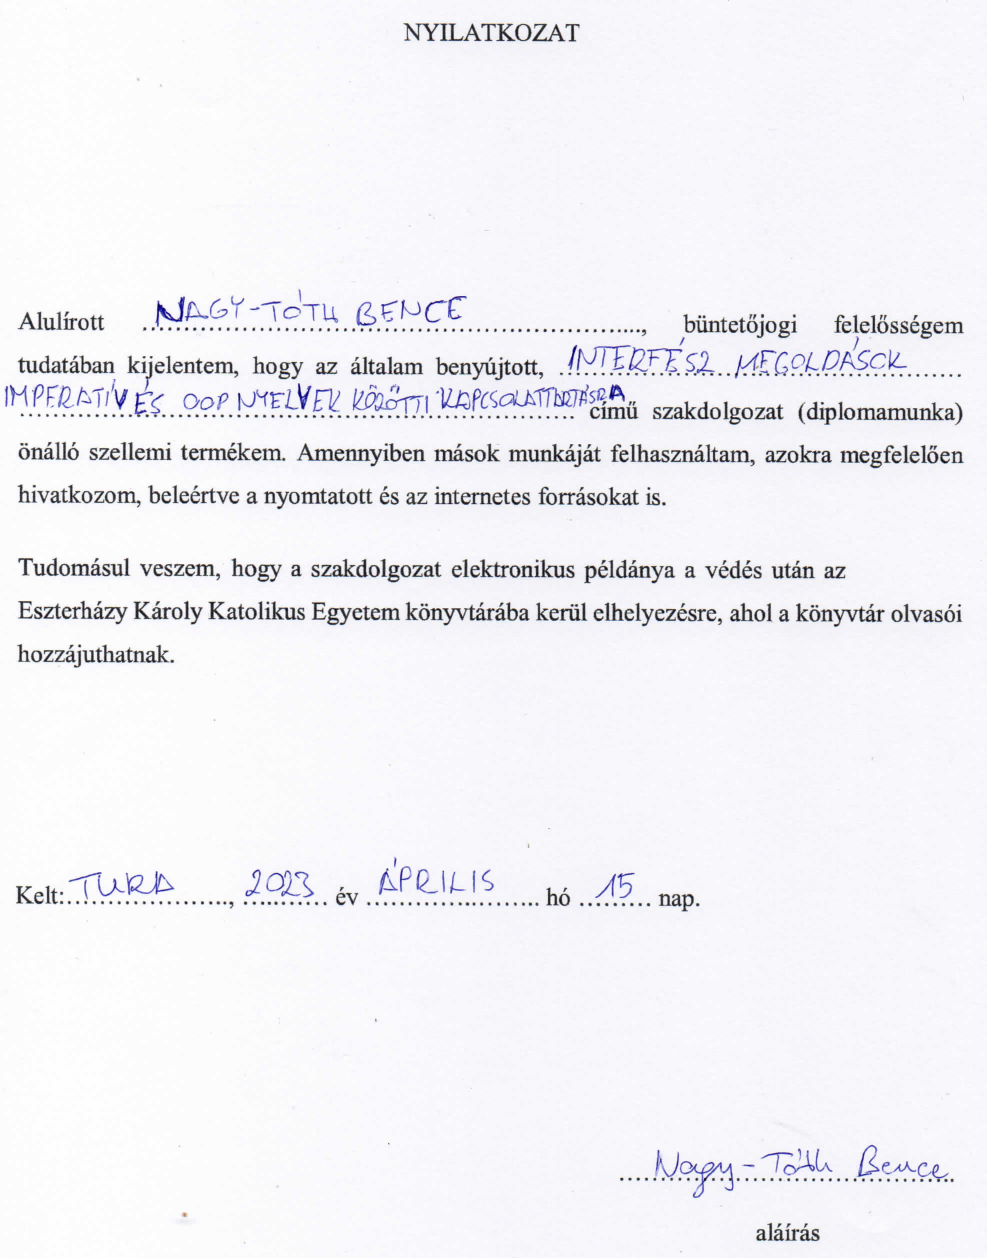
\includepdf{nyilatkozat.pdf}
\end{document}